\subsection{Definition}%
\label{subsec:hgraph_definition}%
Before defining the \ac{hgraph}, some definitions are provided on which the \ac{hgraph} depends. First, recall the \textbf{configuration} definition.\bs

Formally an \textbf{configuration}, $\gls{c}_{id}(k)$ is a tuple of $\left\langle \gls{x}(\gls{k}), \gls{y}(\gls{k}), \gls{theta}(\gls{k})\right\rangle$\\ where $\gls{x}, \gls{y} \in \mathbb{R}, \quad  \gls{theta} \in [0, 2\pi)$\bs

An object is represented as its shape and configuration\\Formally, a \textbf{object},  $\gls{obj}_{id}(\gls{k}) = \left\langle \gls{c}(k), \mathit{shape} \right\rangle $\bs

where $\mathit{shape}$ is linked to a 3D representation of the object, \textit{id} is an identifier for the object.\bs

An object node represents an object in a configuration.\\Formally, a \textbf{objectNode}, $V^{\gls{obj}}_{id} =\left\langle \textrm{status}, \gls{obj}(k)\right\rangle $.\bs

An edge describes how a node transitions to another node in the \ac{hgraph}. In the robot environment, an edge represents an object's configuration change. Edges are split into three categories since they accomplish different goals. \textit{System identification edges} that have as a goal to collect \ac{IO} data and to generate a system model with that data, \textit{action edges} steer a system toward a target configuration and \textit{emtpy edges} connect nodes that contain different objects. The edges are formally defined as:\bs

A \textbf{identification edge}, \[\gls{edge}_{(from, to)} = \left\langle \textrm{status}, id_{from}, id_{to}, \textrm{Identification Method}, \textrm{controller}, \textrm{input}\right\rangle\]\bs

With $id_{from}$ and $id_{to}$ indicating the node identifier where the edge points from and towards, respectively, the identification method indicates the used method, and the controller contains the control method used for driving the robot during the collection of \ac{IO} data. The input contains multiple input sequences to apply to the system. The yielded system model must meet the controller requirements, otherwise, they are incompatible.\bs

A \textbf{action edge}, \[\gls{edge}_{(from, to)} = \left\langle \textrm{status}, id_{from}, id_{to}, \textrm{verb}, \textrm{controller},\textrm{dynamic model}, \textrm{path}\right\rangle\]\bs

With $id_{from}$ and $id_{to}$ indicating the node identifier of the node in the \ac{hgraph} where the edge starts from, and points to, verb is an English verb describing the action the edge represents (driving, pushing), the controller contains the control method used for driving the robot, the dynamic model is the dynamic model used by the control method and the path a list of configurations indicating the path connecting a start- to target node.\bs

A \textbf{empty edge}, \[\gls{edge}_{(from, to)} = \left\langle \textrm{status}, id_{from}, id_{to}\right\rangle\]\bs

Where the status for an emtpy edge can be INITIALIZED or FAILED.\bs

Connecting nodes with edges is eleborated upon in the upcoming section. Two nodes can only be connected if they both contain the same object. The empty edge main goal is to connect nodes that contain different object, to involve multiple objects in a single  action sequence.\bs

Now that the nodes and edges have been defined, the \ac{hgraph} can be defined.\bs

Formally, a \textbf{hypothesis graph}, $\gls{hgraph} = \left\langle \gls{nodesH}, \gls{edgesH} \right\rangle $
\\ Where \gls{nodesH} is a set of nodes and \gls{edgesH} a set of edges, defined as: $\gls{nodesH} = \{\gls{nodesH}^{\gls{obj}}_{i}\}$, \quad $\gls{edgesH} \in \{\gls{edge}_{(i,j)}| \gls{edgesH}_i, \gls{edgesH}_j \in \{\gls{nodesH}^{\gls{obj}} \}, i \neq j\}$.\bs

Most \ac{hgraph} components have been defined. The status of an identification or action edge remains undefined and requires further explanation.\bs

\subsection{Edge statusus}
The edges are split into two categories, identification edges and action edges. An identification edge sends an input sequence and records the system output. That \ac{IO} sequence and assumptions on the system are the basis for system identification, techniques on various system identification methods are discussed in \Cref{sec:sys_iden}. The goal is to create a dynamic model augmented with a corresponding controller that forms closed-loop stable control. The status of an identification edge can be visualized in the following \ac{FSM}.\bs

\begin{figure}[H]
\centering
\begin{tikzpicture}[node distance = 2cm, auto, initial]
    \node [state, fill=my_dark_blue] (init_test_num) {PrIS\#t};
    \node [state, fill=my_light_blue, below of=init_test_num] (completed_test_num) {PoIS\#t};
    \node [state, accepting, fill=my_green, below of=completed_test_num] (completed) {CO};
    \node [state, accepting, fill=my_red, right of=completed_test_num, node distance=6cm] (failed) {FAIL};

 % arrows
    \draw [-stealth] ([xshift=-2cm]init_test_num.west) to node[near start,above]{\shortstack[]{Select compatible\\sys. iden. method\\Go to first $\gls{c}_{\mathit{start}}$}} (init_test_num.west);
    \draw[-stealth] (init_test_num) edge[bend right] node[left]{Collect \ac{IO} data} (completed_test_num)
(completed_test_num) edge node[left]{Create system model} (completed);
    \draw [-stealth] (completed_test_num) edge[bend right] node[right]{\shortstack{Go to next\\start configuration}} (init_test_num);
    \draw [-stealth] (completed_test_num) to node[below]{\shortstack[]{Unable to reach next\\start configuration}}  (failed.west);
    % \draw [-stealth] (init_test_num) [out=0, in=90] to node[above]{Unable to reach starting robot configuration}  (failed.north);

\end{tikzpicture}
\caption{\acl{FSM} displaying the status of an identification edge}%
\label{tikz:status_identification_edge}
\end{figure}

\noindent
\begin{table}[H]
\centering
\begin{tabular}%
  {>{\raggedleft\arraybackslash}p{0.30\textwidth}%
   >{\raggedright\arraybackslash}p{0.60\textwidth}}
PRE INPUT SEQUENCE number t (PrIS\#t): & Go to target configuration to apply the input sequence. \\
POST INPUT SEQUENCE number t (PoIS\#t): & Collect the output sequence. \\
COMPLETED (CO): & The edge has driven the system toward its target configuration, and its performance has been calculated. \\
FAILED (FAIL): & An error occurred, yielding the edge unusable. \\
\end{tabular}
\end{table}

An identification edge corresponds to an action edge because its goal is to generate a system model to hand over its corresponding action edge. The system identification method is selected after the action edge is selected to yield a system model compatible with the controller that resides in the action edge. Two types of system models are generated: system models that describe the driving behaviour of the robot and system models that describe the robot's push behaviour and an object's.\bs

After initialization, an action edge starts propagating its status as indicated in \Cref{tikz:status_action_edge}. An action edge's eventual goal is to track a path. First, the existence of a path is estimated, a system model must be provided, and action planning must be performed. \bs

\begin{figure}[H]
\centering
\begin{tikzpicture}[node distance = 2cm, auto, initial]
    \node [state, fill=my_purple] (init) {IN};
    \node [state, fill=my_dark_blue, below of=init] (path_exist) {PE};
    \node [state, fill=my_light_blue, below of=path_exist] (system_model) {SM};
    \node [state, fill=my_green, below of=system_model] (path_planned) {PP};
    \node [state, fill=my_yellow, below of=path_planned] (executing) {EX};
    \node [state, accepting, fill=my_orange, below of=executing] (completed) {CO};
    \node [state, accepting, fill=my_red] (failed) at ([xshift=4cm]$(system_model)!0.5!(path_planned)$) {FAIL};

 % arrows
    \draw [-stealth] ([xshift=-2cm]init.west) to node[near start,above]{Select controller} (init.west);
    \draw[-stealth] (init) edge node[left]{Graph-based path estimation} (path_exist)
      (path_exist) edge[bend right] node[left]{Load in system model} (system_model)
(system_model) edge[bend right] node[left]{Path planning} (path_planned)
(path_planned) edge[bend right] node[left]{Go to execution loop} (executing)
(executing) edge[bend right] node[left]{Completed} (completed);

    \draw [-stealth] (init.east) [out=0, in=90] to node[xshift=0.1cm, right]{Path non-existence proven}  ([yshift=-0.03cm,xshift=0.2cm]failed.north);
    \draw [-stealth] (path_exist.east) [out=0, in=90] to node[xshift=-0.6cm,yshift=0.55cm, above]{\shortstack[l]{System\\identification\\error}}  ([yshift=-0.03cm,xshift=-0.2cm]failed.north);
    \draw [-stealth] (system_model.east) [out=0, in=180] to node[xshift=0.1cm, yshift=0.3cm, above]{\shortstack[l]{Path\\planning\\error}} (failed.west);
    node[right]{path planning error}
    ([yshift=-0.3cm]failed.west);
    \draw [-stealth] (executing.east) [out=0, in=-90] to node[xshift=0.1cm,right]{Fault detected}(failed.south);

\end{tikzpicture}
\caption{\acl{FSM} displaying the status of an action edge}%
\label{tikz:status_action_edge}
\end{figure}

\noindent
\begin{table}[H]
\centering
\begin{tabular}%
  {>{\raggedleft\arraybackslash}p{0.24\textwidth}%
   >{\raggedright\arraybackslash}p{0.66\textwidth}}
INITIALIZED (IN): & The edge is created with a source and target node, which are present in the \ac{hgraph}. A choice of controller is made by random selection. \\
PATH EXISTS (PE): & A graph-based search is performed to validate whether the target configuration is reachable, assuming the system is holonomic. \\
SYSTEM MODEL (SM): & A dynamics system model is provided to the controller residing in the edge. \\
PATH PLANNED (PP): & Resulting from a sample-based planner, a path from start to target configuration is provided. \\
EXECUTING (EX): & The edge receives observations from the robot environment and sends back robot input. \\
COMPLETED (CO): & The edge has driven the system toward its target configuration, and its performance has been calculated. \\
FAILED (FAIL): & An error occurred, yielding the edge unusable. \\
\end{tabular}
\end{table}


\subsection{Legend}
\todo{hmmm, you want this?}

\Cref{tikz:status_action_edge} shows that many steps must successfully be completed before the edge can be executed.
Before executing edges, edges must be initialized, which is where the next section is dedicated to.\bs

The following figure presents an legend for the \ac{hgraph}s that will be presented in the next section.\bs

\begin{figure}[H]
    \centering
    \begin{subfigure}{0.2\textwidth}
    \centering
    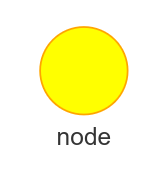
\includegraphics[width=0.7\textwidth]{figures/proposed_method/connecting_nodes/legend/node}
    \caption{Regular node created by the \ac{halgorithm}.\newline}%
    \end{subfigure}
    \begin{subfigure}{0.2\textwidth}
    \centering
    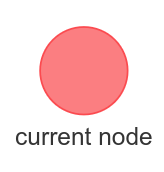
\includegraphics[width=0.7\textwidth]{figures/proposed_method/connecting_nodes/legend/current_node}
    \caption{Current node indicates that its outgoing edge is or is next to be executed.}%
    \end{subfigure}
    \begin{subfigure}{0.2\textwidth}
    \centering
    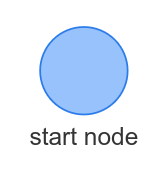
\includegraphics[width=0.7\textwidth]{figures/proposed_method/connecting_nodes/legend/starting_node}
    \caption{Starting node, one is generated at for every subtask.}%
    \end{subfigure}
    \begin{subfigure}{0.2\textwidth}
    \centering
    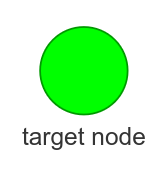
\includegraphics[width=0.7\textwidth]{figures/proposed_method/connecting_nodes/legend/target_node}
    \caption{Target node, one is generated for every subtask.\newline}%
    \end{subfigure}

    \begin{subfigure}{0.33\textwidth}
    \centering
    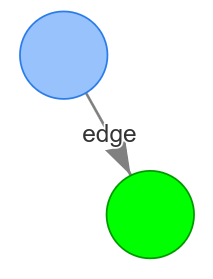
\includegraphics[width=0.7\textwidth]{figures/proposed_method/connecting_nodes/legend/edge}
    \caption{Edge with status IN, PE, SM, PP or EX.}%
    \end{subfigure}
    \begin{subfigure}{0.33\textwidth}
    \centering
    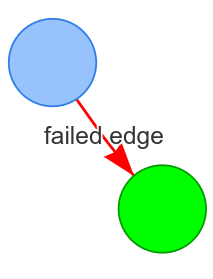
\includegraphics[width=0.7\textwidth]{figures/proposed_method/connecting_nodes/legend/failed_edge}
    \caption{Edge with status FAILED (FAIL)}%
    \end{subfigure}
    \begin{subfigure}{0.33\textwidth}
    \centering
    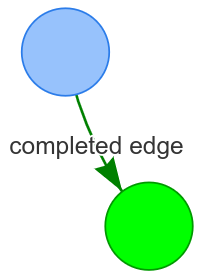
\includegraphics[width=0.7\textwidth]{figures/proposed_method/connecting_nodes/legend/completed_edge}
    \caption{Edge with status COMPLETED (CO)}%
    \end{subfigure}
    \caption{Legend for the \acl{hgraph}. }%
    \label{fig:hgraph_legend}
\end{figure}
